\label{sec::results}
\subsection{Quantum Steering Efficacy}
	\label{sec::steering}
\todo[inline]{Discuss all results related to nuclear spin mapping}

	As discussed in \hyperref[sec::nuc_spin_map]{section \ref{sec::nuc_spin_map}}, nuclear spin mapping was used to improve the readout fidelity of our experiment. However, the improvement in fidelity was conditional upon the initial state of the electron at the time of the mapping. To perform correct mapping, a spin-down electron is required. To measure the fidelity of the nuclear mapping, and implicitly the quantum steering efficacy, the state of the nucleus was measured for many steering times, and repeated to minimise the limits of accuracy in the measurement. Figure \ref{fig::wait_time} shows the total experimental error as a function of steering time. As steering time increases, we are more confident that the state of the electron was spin-down at the time of mapping, which is reflected in our decrease in error. The average time spent in the initialisation period is plotted on the right-axis. This would exceed the steering time in the average case, as a blip in current would require postponement of the donor plunge.	There are 2 separate data sets plotted one for each $B = 1.4$ T and $B = 1$. For $B = 1.4$ T, there were 2000 nuclear readouts per data point and for $B = 1.0$ T there were 500 nuclear readouts.
	
	\begin{figure}[htbp!]
		\centering
		\vspace{-1cm}
		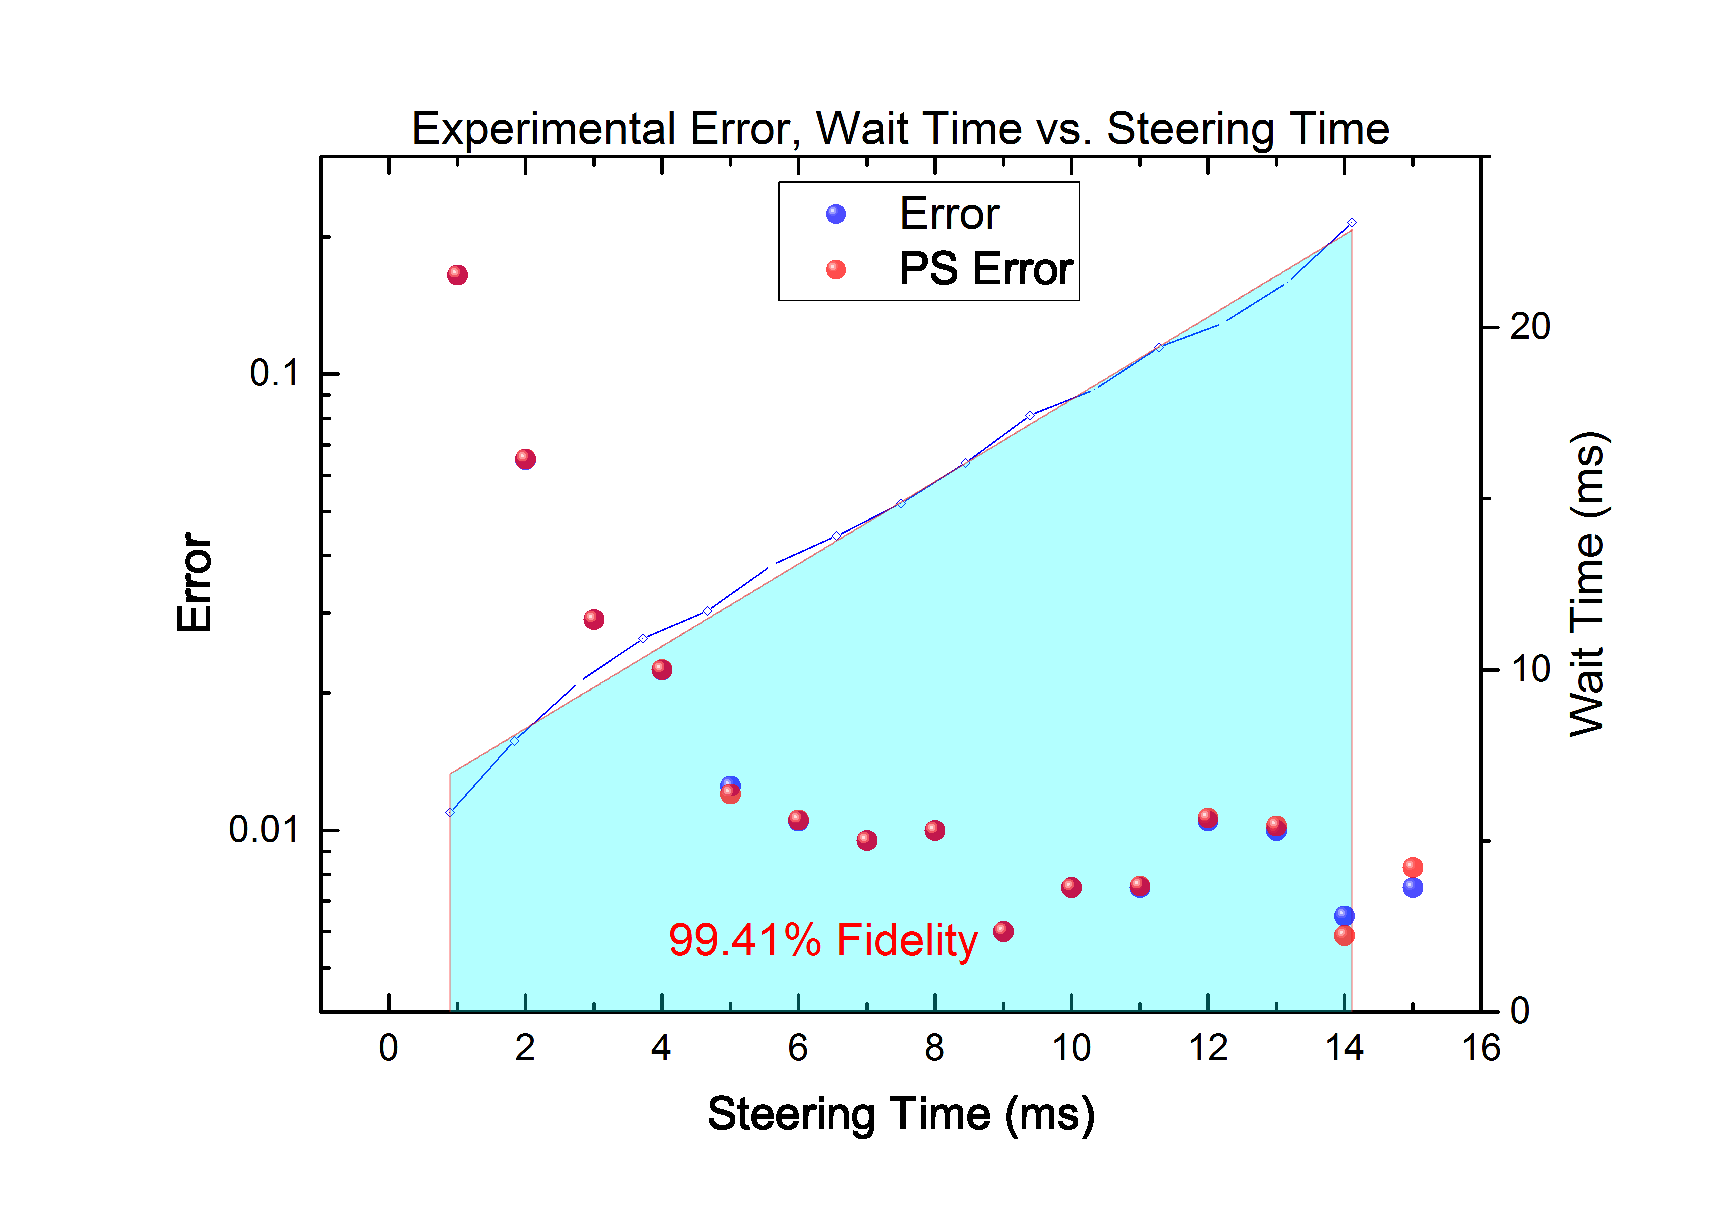
\includegraphics[width=\textwidth]{WaitTimeFigLog_1p4T}
		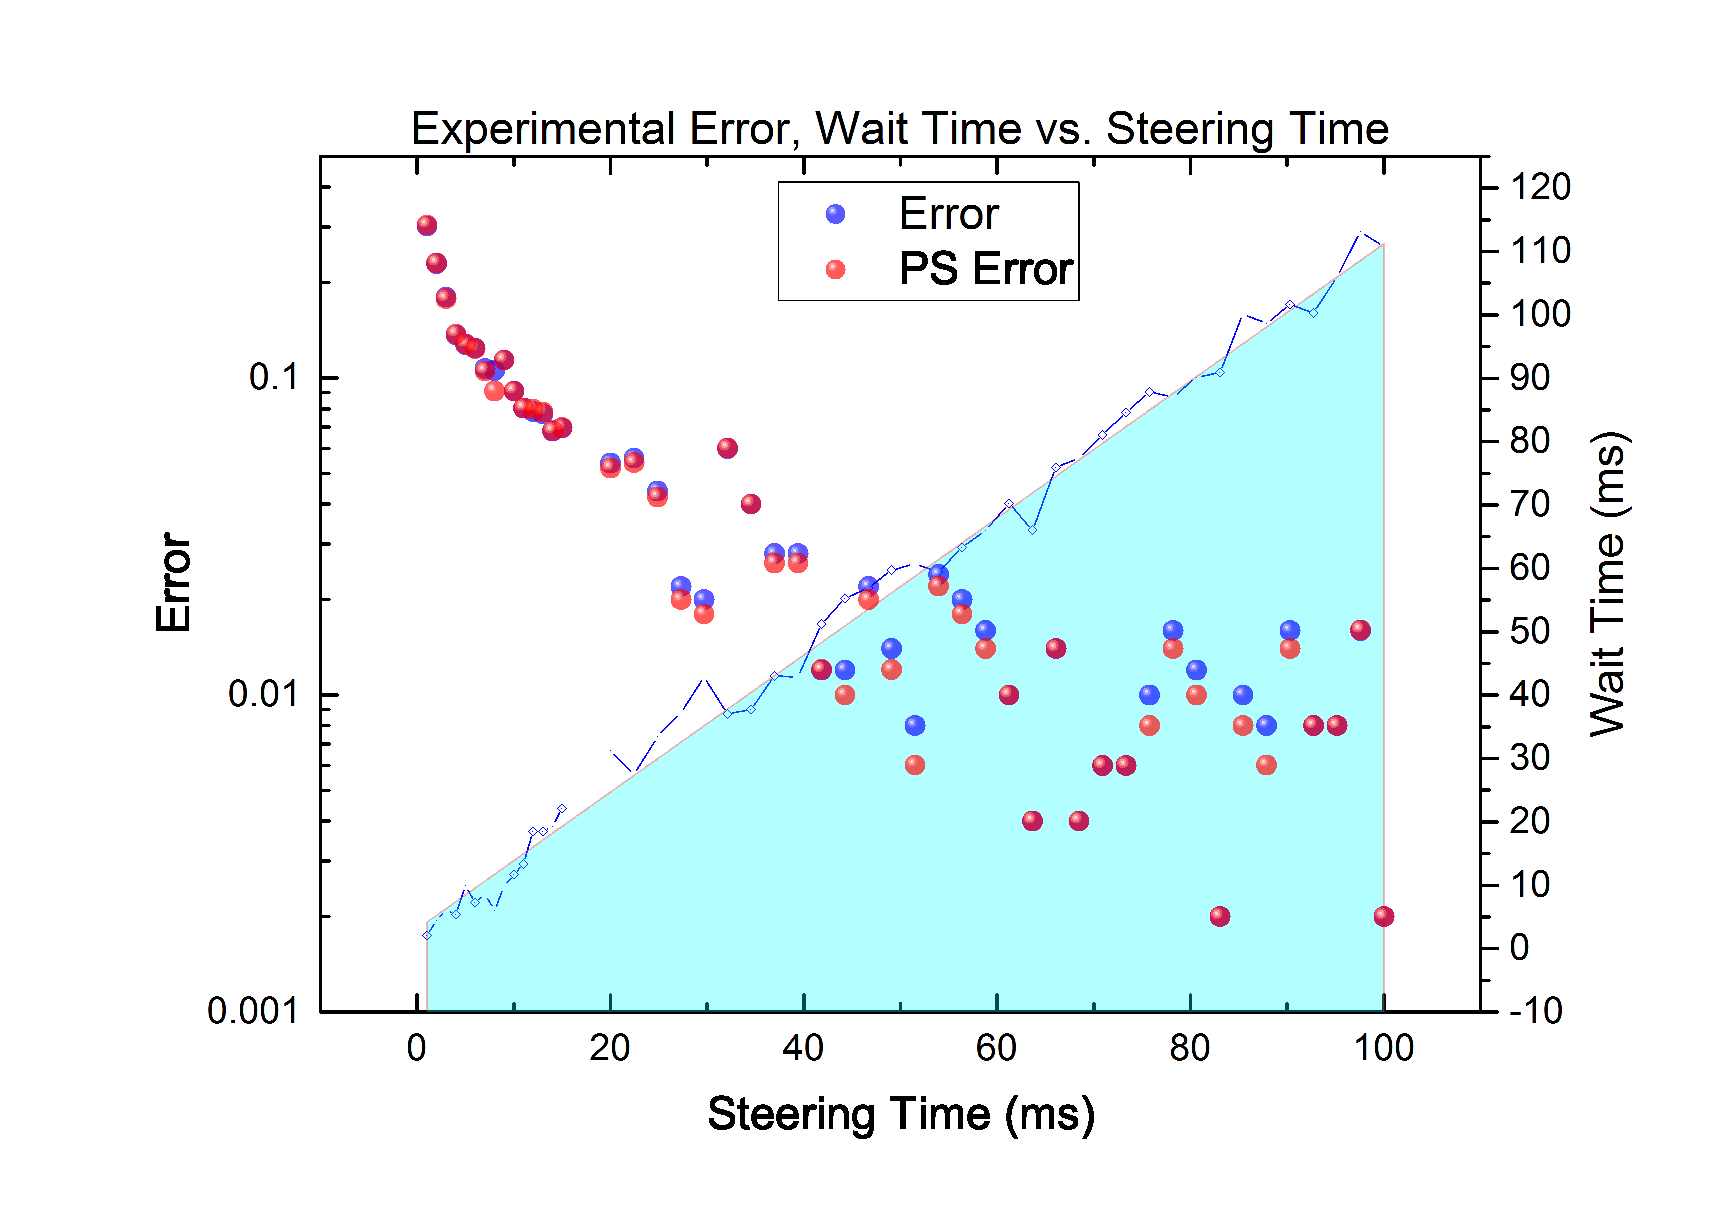
\includegraphics[width=\textwidth]{WaitTimeFigLog_1p0T}
		\caption[Experimental fidelity with varying steering times.]{For a field of $B = 1.4$ T (top) and $B = 1.0$ T (bottom), the experimental error is plotted against steering time. On  the right axis is the average time spent at the initialisation level during the experiment.}
		\label{fig::wait_time}
	\end{figure}
		
	These two datasets show the relationship between the required steering time for a good initialisation and the apparent tunnelling time of the donor electron. As expected, with a larger steering time the fidelity of the experiment approaches 100\% following an exponential decay, determined by the characteristic tunnel time. In each plot of Figure \ref{fig::wait_time}, there are two sets of points plotted, raw error data given by analysing all nuclear flips and PS error, or post-selection error, where readouts that were initialised poorly are ignored. Poor initialisation will be explained and explored in \hyperref[sec::latency]{Section \ref{sec::latency}}. Post-selecting improves the experimental fidelity, as we remove cases which are likely to be cause an incorrect nuclear mapping, and it has been shown that with post-selection the experimental fidelity can reach 99.9\% \todo{somehow give citation to Stef, no paper on this though}, though, in these plots, the maximum is constrained by the limits of accuracy for the measurement, which was 0.2\% (500 readouts), and hence the maximum observed fidelity is 99.8\%.

	This result exactly demonstrates the effect of quantum steering as a method for filtering incorrect initialisation through quantum-back action. The results mirror those presented in Section \ref{sec::spin_init}.
	
	The required steering time to achieve 99\% fidelity is much longer for $B = 1$ T, however it was observed that the average tunnel time had not increased by such a margin from $B = 1.4$ T. This could be explained if we accept that the probability of a spin-down electron tunnelling off during the initialisation phase is high (also known as a dark-count), which is physically the same as a read-error. Whilst this is a possible explanation, it's not clear if this is accurate, and more examination of the data is required. All approximations made of a simple exponential decay have assumed that the dark-counts are negligible.

\subsection{Nuclear and Electron Rabi Oscillations}
	\todo[inline]{Discuss results pertaining to a high fidelity readout from a nuclear/electron rabi}
	A nuclear Rabi oscillation was performed by loading an electron onto the donor, followed my mapping the state onto the nucleus. This electron is ideally spin-down for this step. After the nucleus is prepared, we stimulate it with an \gls{rf} pulse of duration $\tau_{RF}$, which is swept as part of the experiment. After the \gls{rf} exposure, we then map the nucleus state back onto an electron using another \gls{mw} pulse, followed by a readout of the electron state. We perform 20 repeated measures of the nuclear state via the electron in this manner. 	Figure \ref{fig::nuclear_rabi} shows the results of two separate Rabi oscillations, one with electron initialisation by steering, and one without.
	
	
	As we vary $\tau_{RF}$, we observe that the expected value of the nuclear-spin readout, via the electron readout, follows a sinusoid with a frequency known as the Rabi frequency. Arbitrary rotations are a key part of a universal quantum computer, and naturally improving the initialisation fidelity can enable finer rotations to be resolved in readout.
	
	\begin{figure}[H]
		\centering
		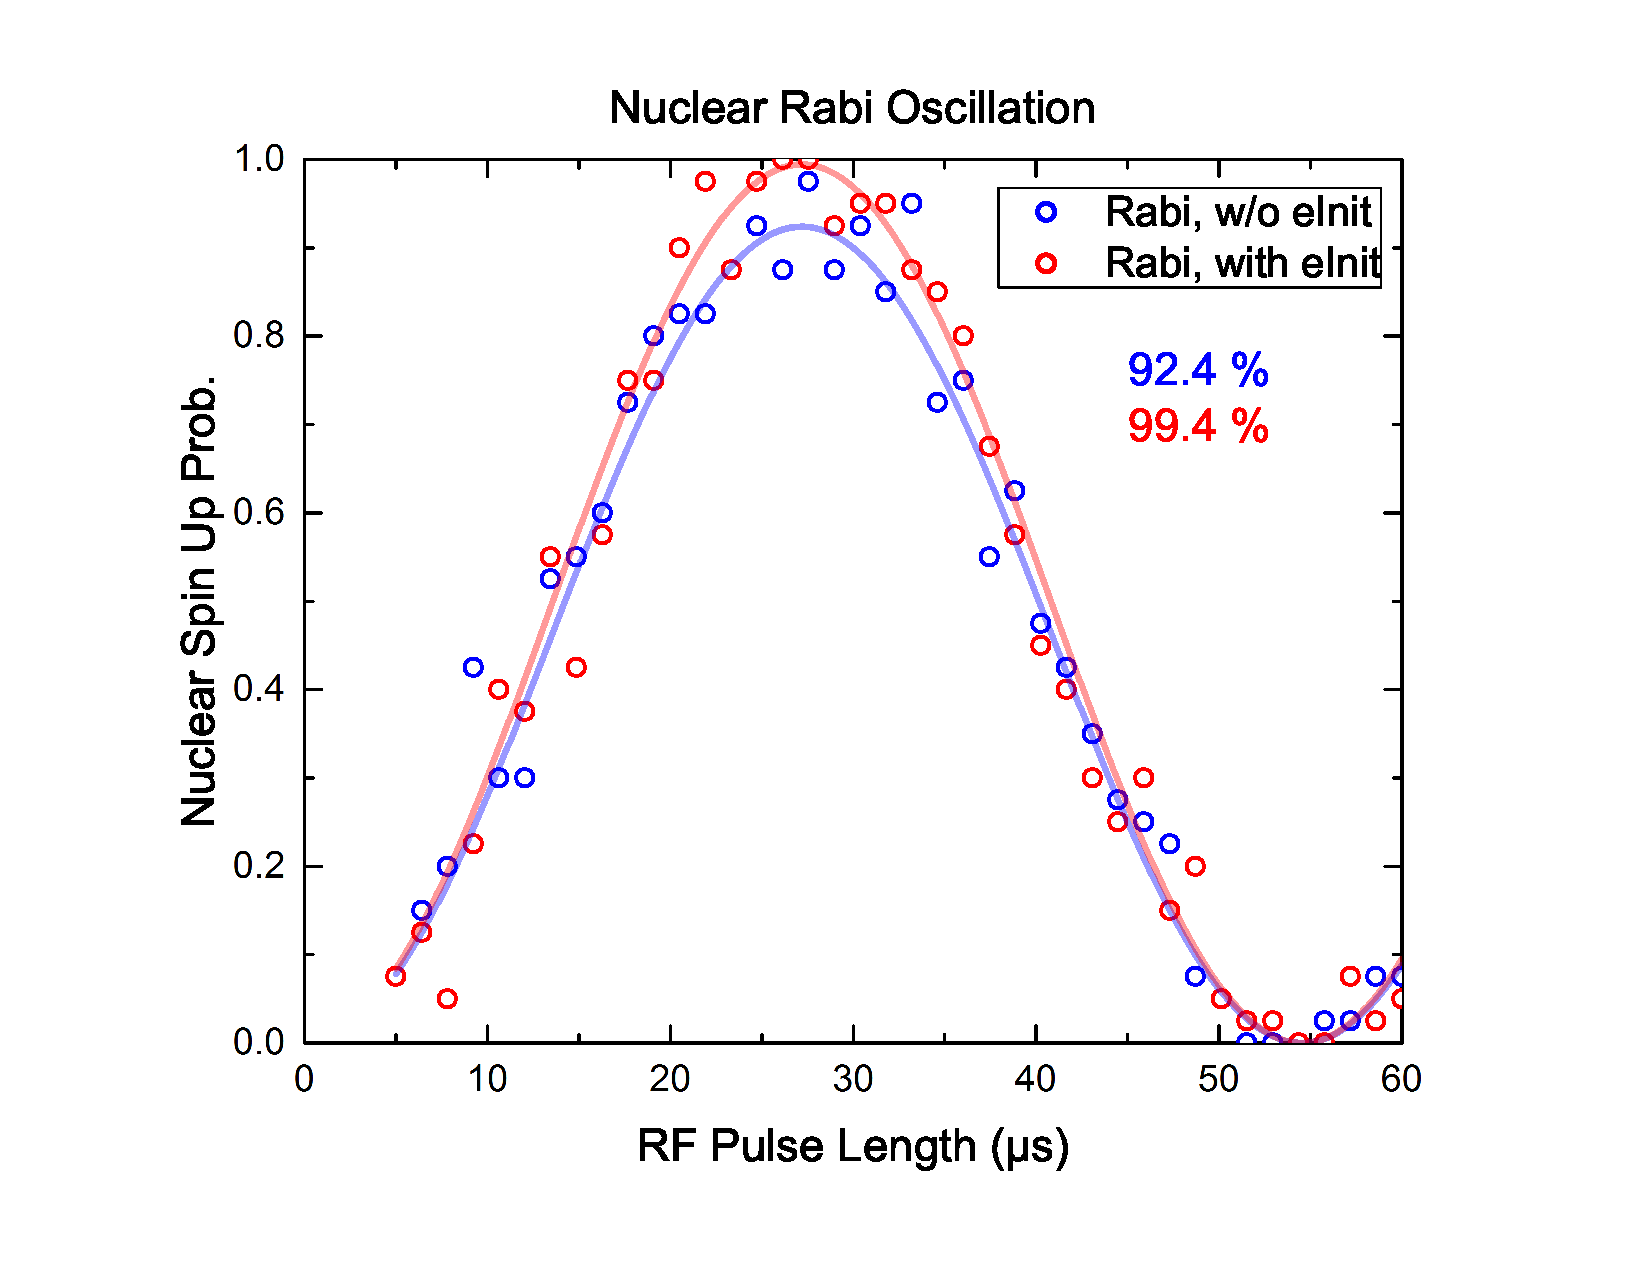
\includegraphics[width=0.8\textwidth]{nRabiFig}
		\caption{A nuclear Rabi oscillation with and without electron initialisation.}
		\label{fig::nuclear_rabi}
	\end{figure}
	
	If we have poor initialisation, this will affect the fidelity of our readout and would reduce the height of the peaks, as shown by the maximum of the fitted sine wave reaching only 92.4\% without initialisation, compared to 99.4\% with initialisation.

\subsection{Initialisation Level Tuning}
	The initialisation level of the pulse sequence was tuned to find the best position for a high fidelity experiment. It was discovered, however, that with initialisation there was a broad  flat-band (approximately 400 mV) in which high fidelity results were obtained. This indicates another benefit in performing electron initialisation, which is insensitivity to tuning. This is a very useful property for a quantum computer, as reproducibility of measurements is crucial in determining the result of a computation.
	
	Figure \ref{fig::initLevel} shows the error rate as a function of initialisation level. As the initialisation level changes, the donor potential will also change about the Fermi level of the reservoir, leading to changes in load and read errors, as explained in Section \ref{sec::load_error}. To reiterate, if the potential of both a spin-up and spin-down electron is such that both have available energy states in the reservoir, they can both tunnel out. If the Zeeman splitting of the donors is much larger than the thermal energy of the system, then we would expect a fairly large region in which to tune the initialisation level, while maintaining spin-dependent tunnelling. 
%	Typically, $ k_B T \ll h \nu_{e2}$, where $k_B, T$ are Boltzmann's constant and the device temperature, respectively.
	By sweeping the initialisation level we observe a cut-off region, greater than approximately 0 V, where the experimental fidelity drops completely. On the negative end of the scale, there appears to be an exponential drop in fidelity, as read errors begin to occur more frequently. Read errors increase as a negative bias shifts the donor potential above the Fermi level, bringing more available states to the level of a spin-down electron.
	
	It is expected that if the steering time is increased, the drop off due to increasing read-errors will diminish, as the steering window will filter more tunnel events. This has not been explored in this thesis.
	
	\begin{figure}[htbp!]
		\flushleft
		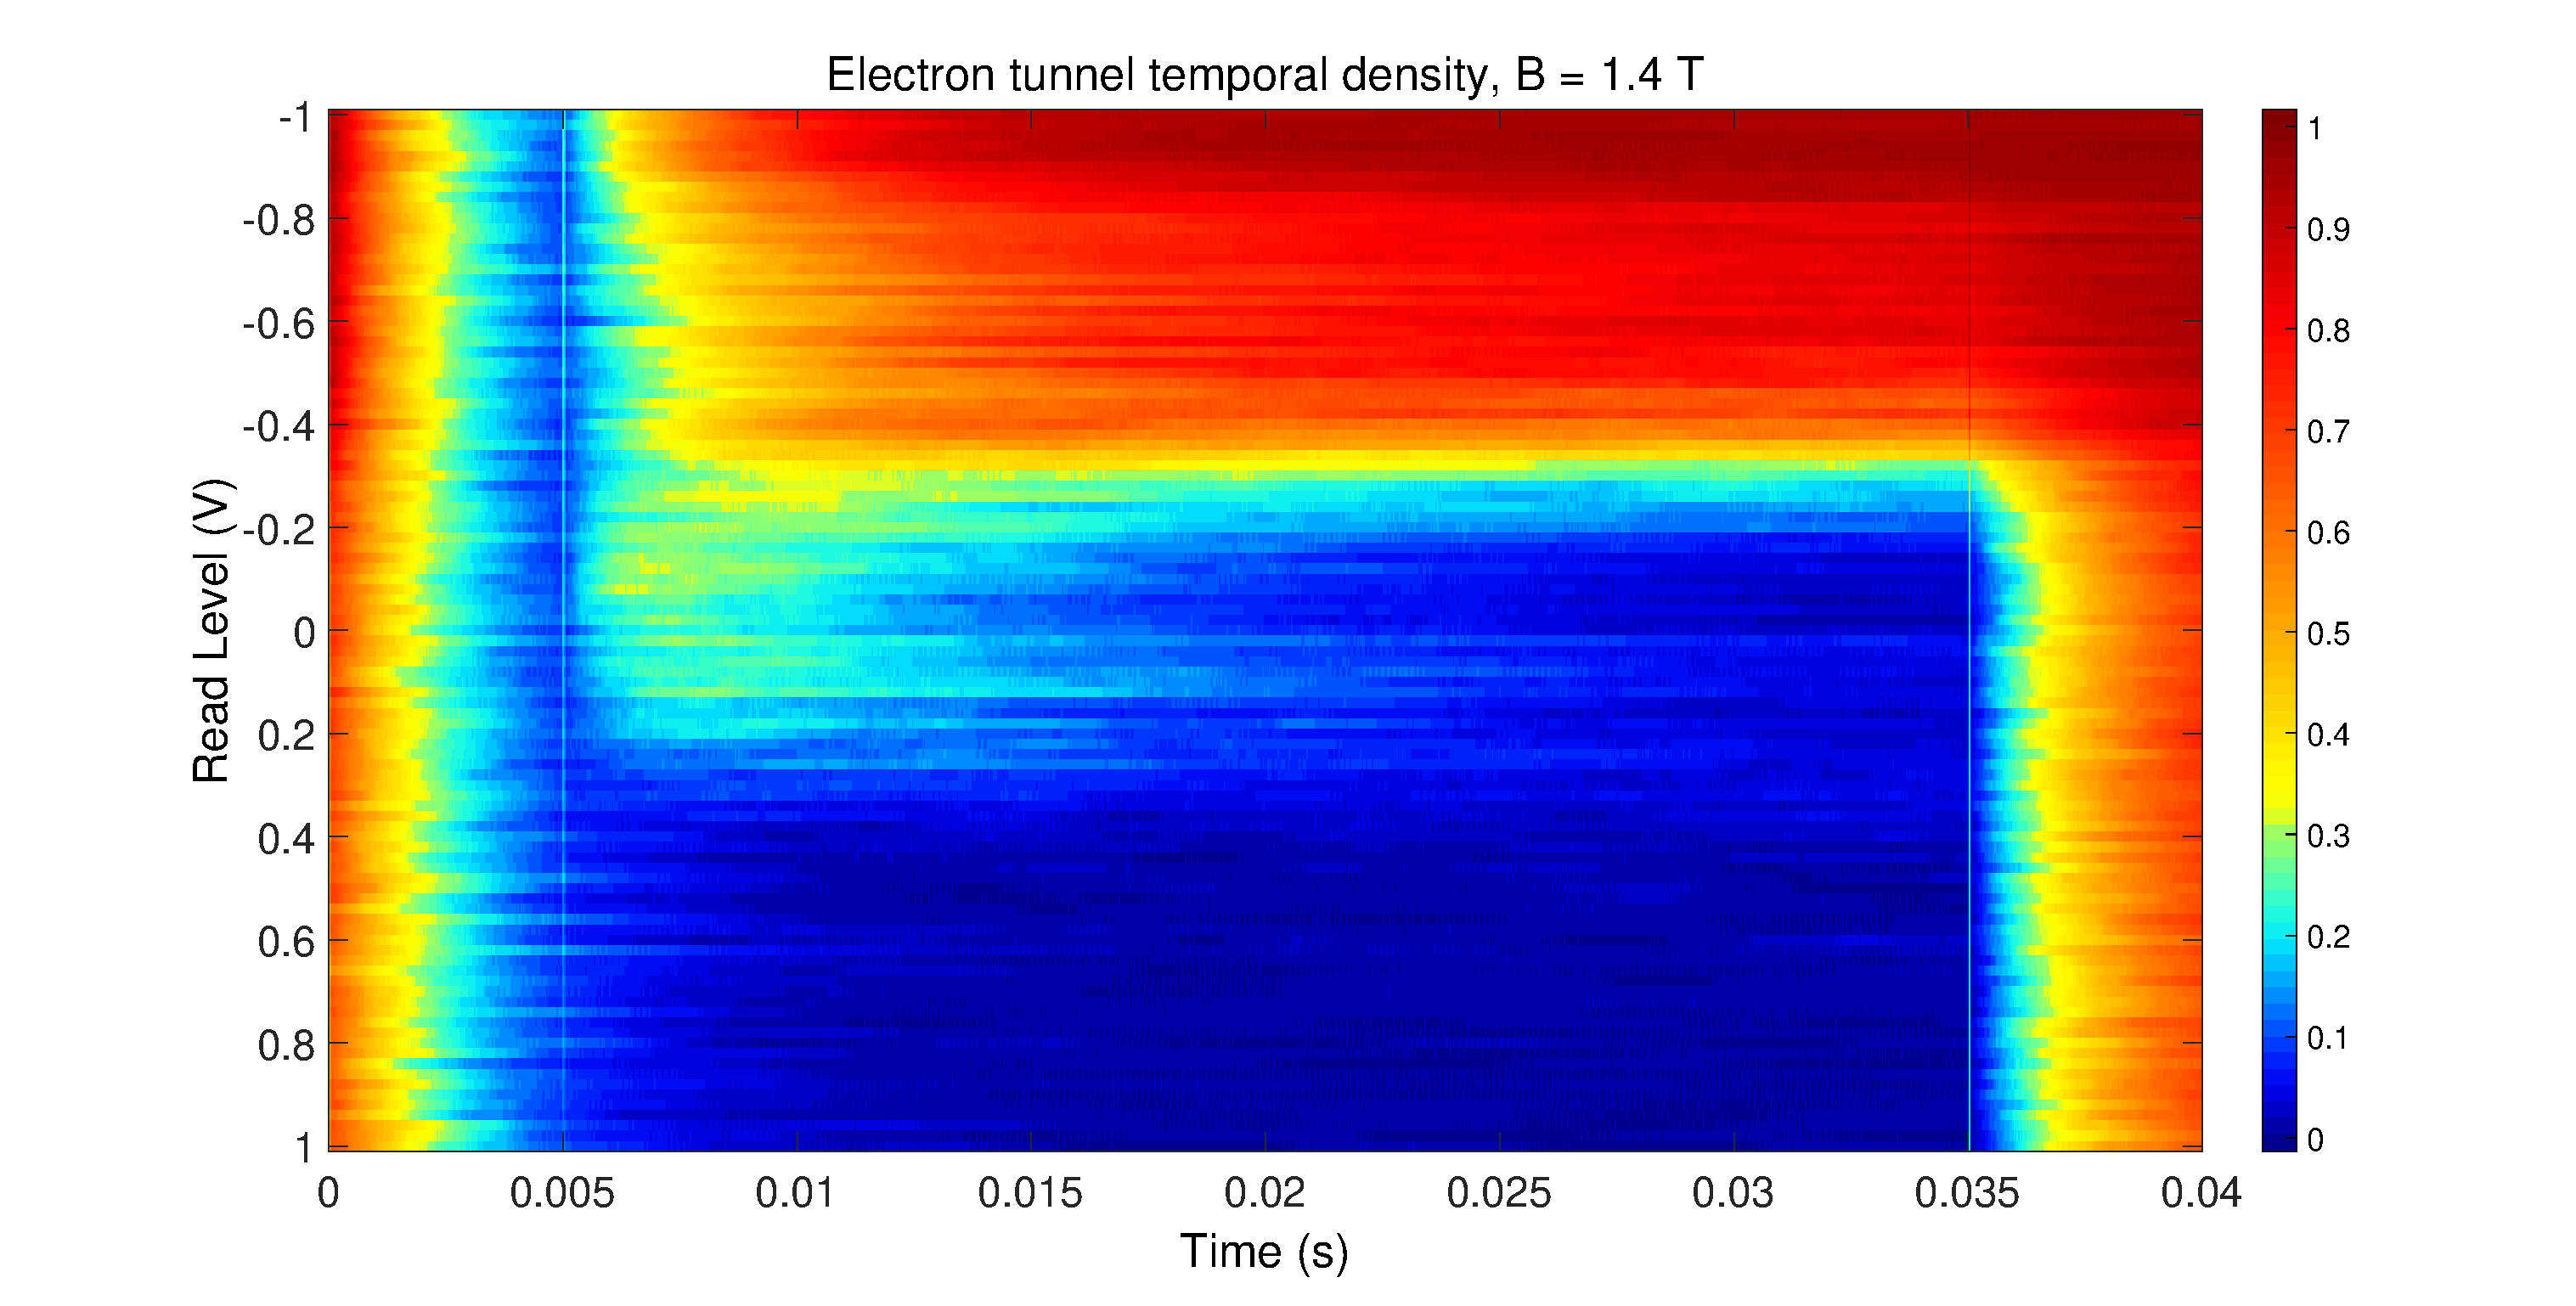
\includegraphics[width=\textwidth,height=0.4\textheight]{readLevelScan_1p4T}
		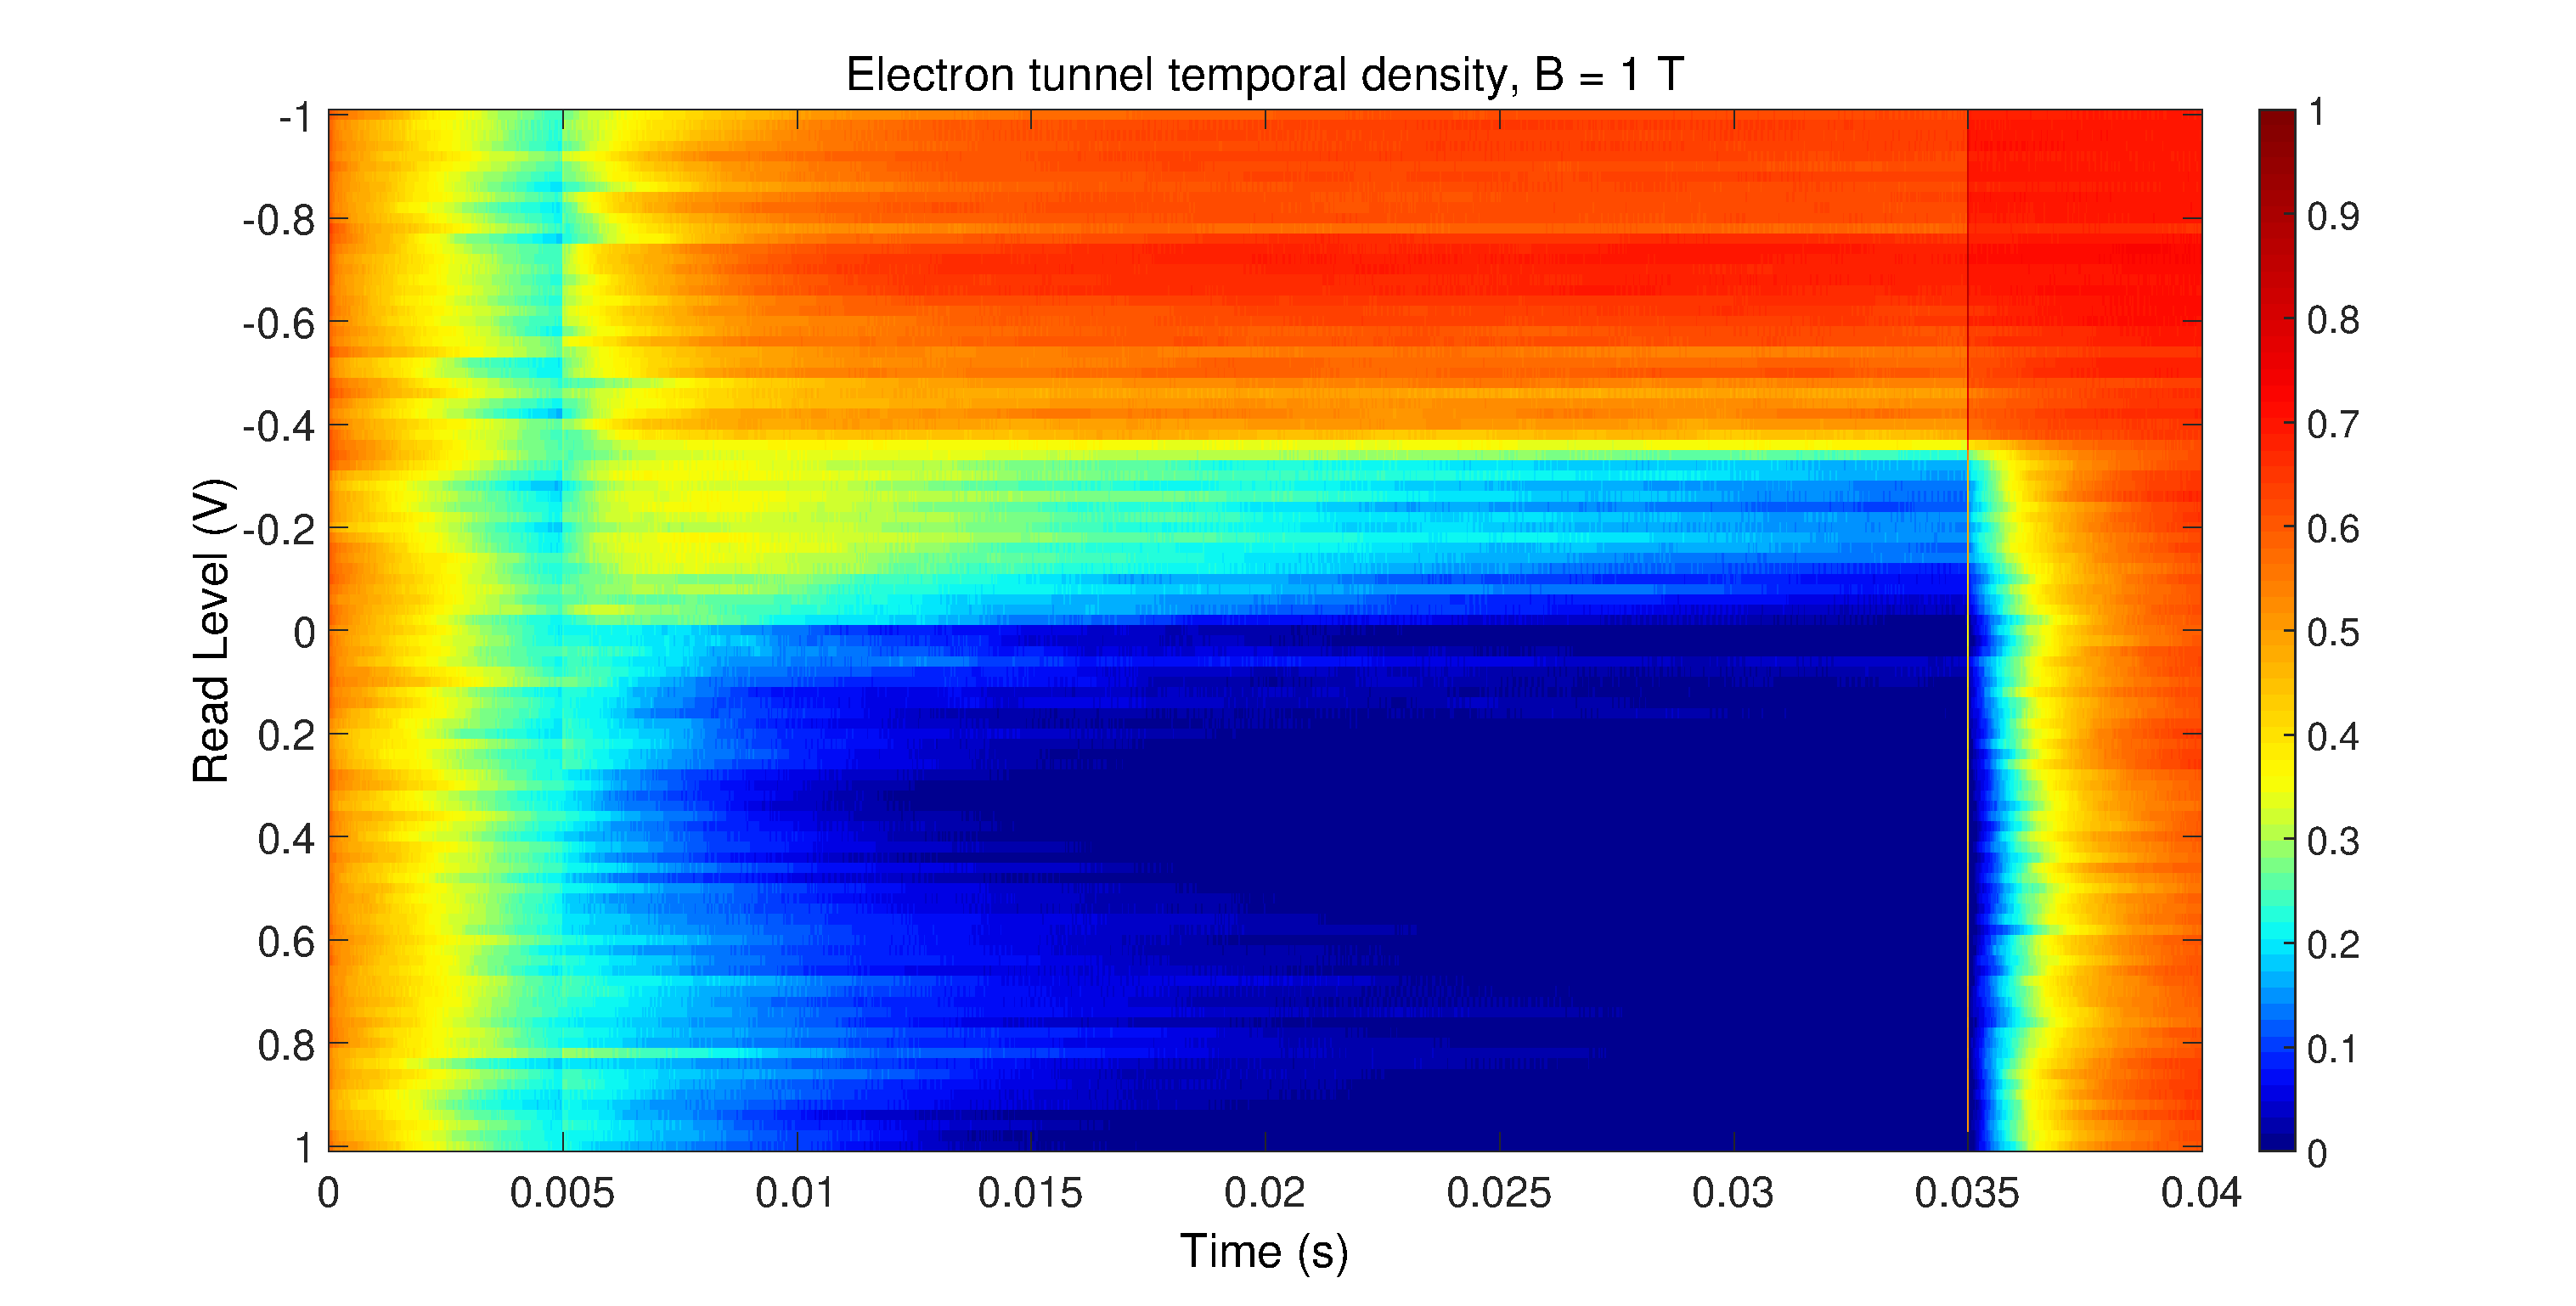
\includegraphics[width=\textwidth,height=0.4\textheight]{readLevelScan_1p0T}
		\caption[Read level scan for two magnetic biases]{For a field of $B = 1.4$ T (top) and $B = 1.0$ T (bottom), the tail of a read level scan is plotted, where red indicates a high current through the \gls{set} while blue indicates low current. The values are average over many runs. 
		Above a certain threshold, the donor will remain ionised and current will continue to flow throughout the load-read-empty cycle. Below a certain threshold the opposite will occur, where any electron on the donor will remain on the donor with high probability, regardless of its spin-state.
		Spin-dependent tunnelling occurs in the mid-region which appears blue-green. 
		}
		\label{fig::readLevel}
	\end{figure}
	
	\begin{figure}[htbp!]
		\centering
		\includegraphics[width=\textwidth]{initLevelFigLog}
		\caption{Experimental error was measured at varied initialisation levels.}
		\label{fig::initLevel}
	\end{figure}
	
	A novel application of this measurement is that we can infer the donor temperature from the width of the flat-band. The flat-band itself is a measure of the tail reading from Figure \ref{fig::readLevel} due to the Zeeman splitting of the electron donor, assuming finite temperature. 

\subsection{Improper Initialisation due to Trigger Latency}
	\label{sec::latency}
	Due to the nature of a software solution, there is an inherent latency between making a decision in software, and triggering hardware to react. The effect of this is shown in Figure \ref{fig::latency}, where the donor became ionised before the plunge, and so there was no electron to be initialised and the result must be discarded. There are two possibilities that occur due to this latency, the first being plunging when the donor is ionised and therefore potentially not being able to perform a spin-mapping. The second is if the donor ionises and deionises in this latency window, meaning there is an electron to map to the nucleus but it is in an indeterminate state.
	
	\begin{figure}[htbp!]
		\centering
		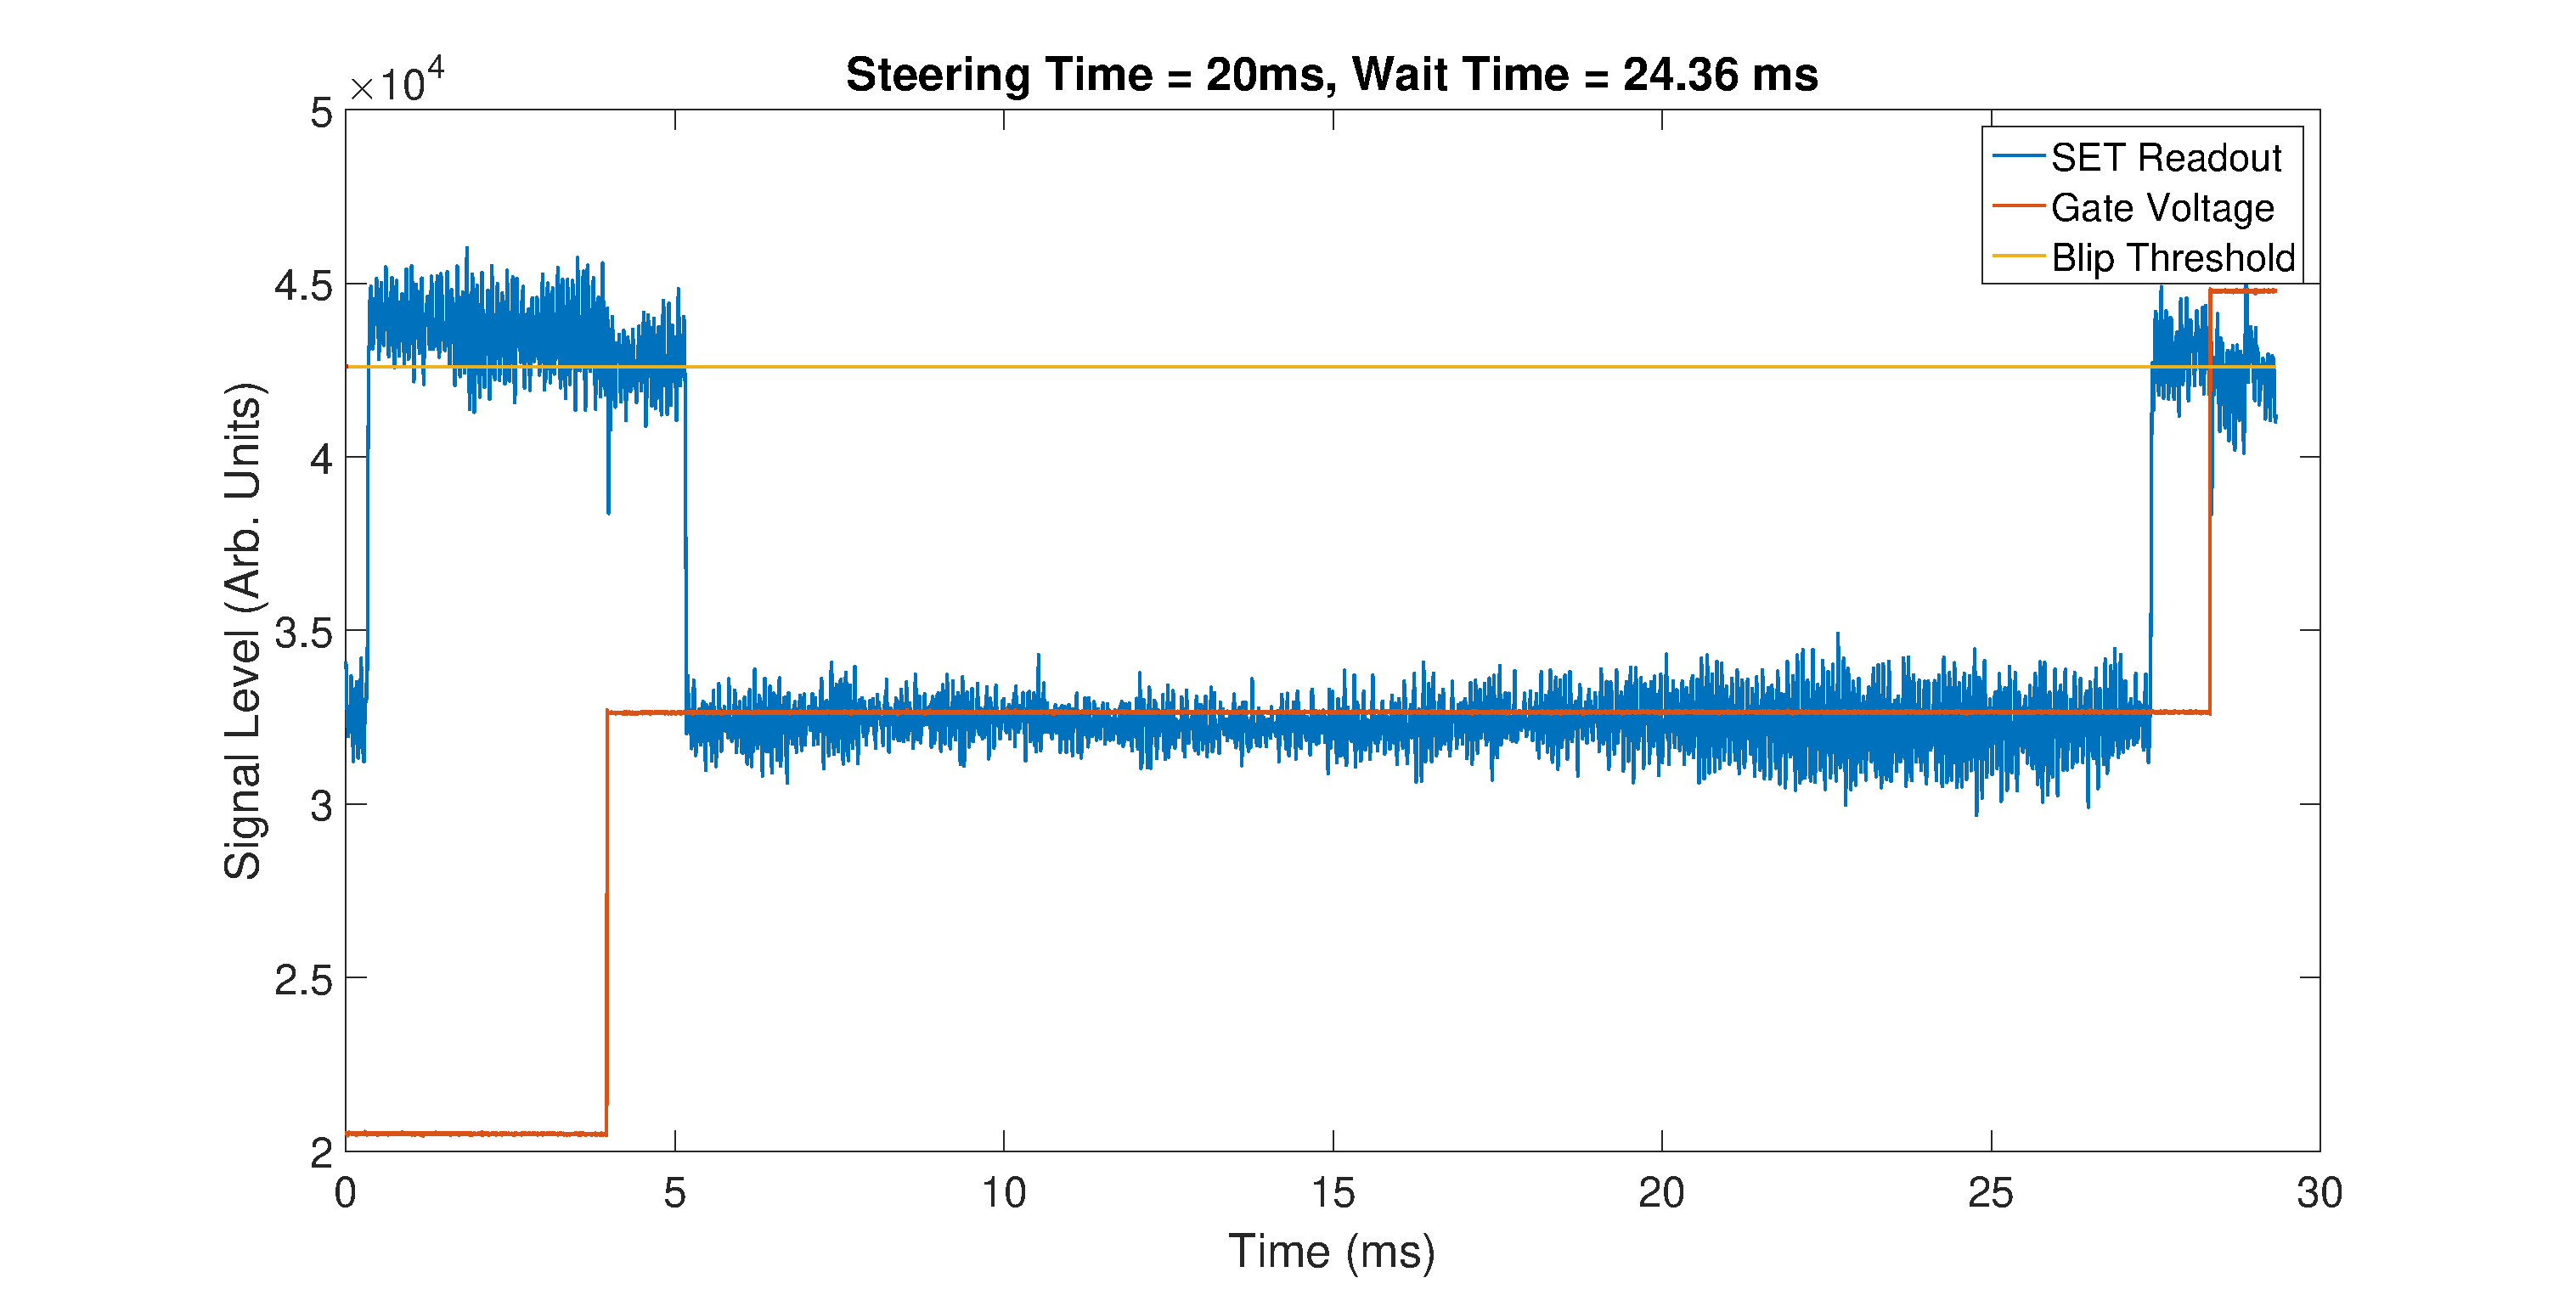
\includegraphics[width=\textwidth]{MATLAB_latency}
		\caption{Improper initialisation occurs due to a latency in the trigger sent by MATLAB.}
		\label{fig::latency}
	\end{figure}
	
	\begin{figure}[htb!]
		\centering
		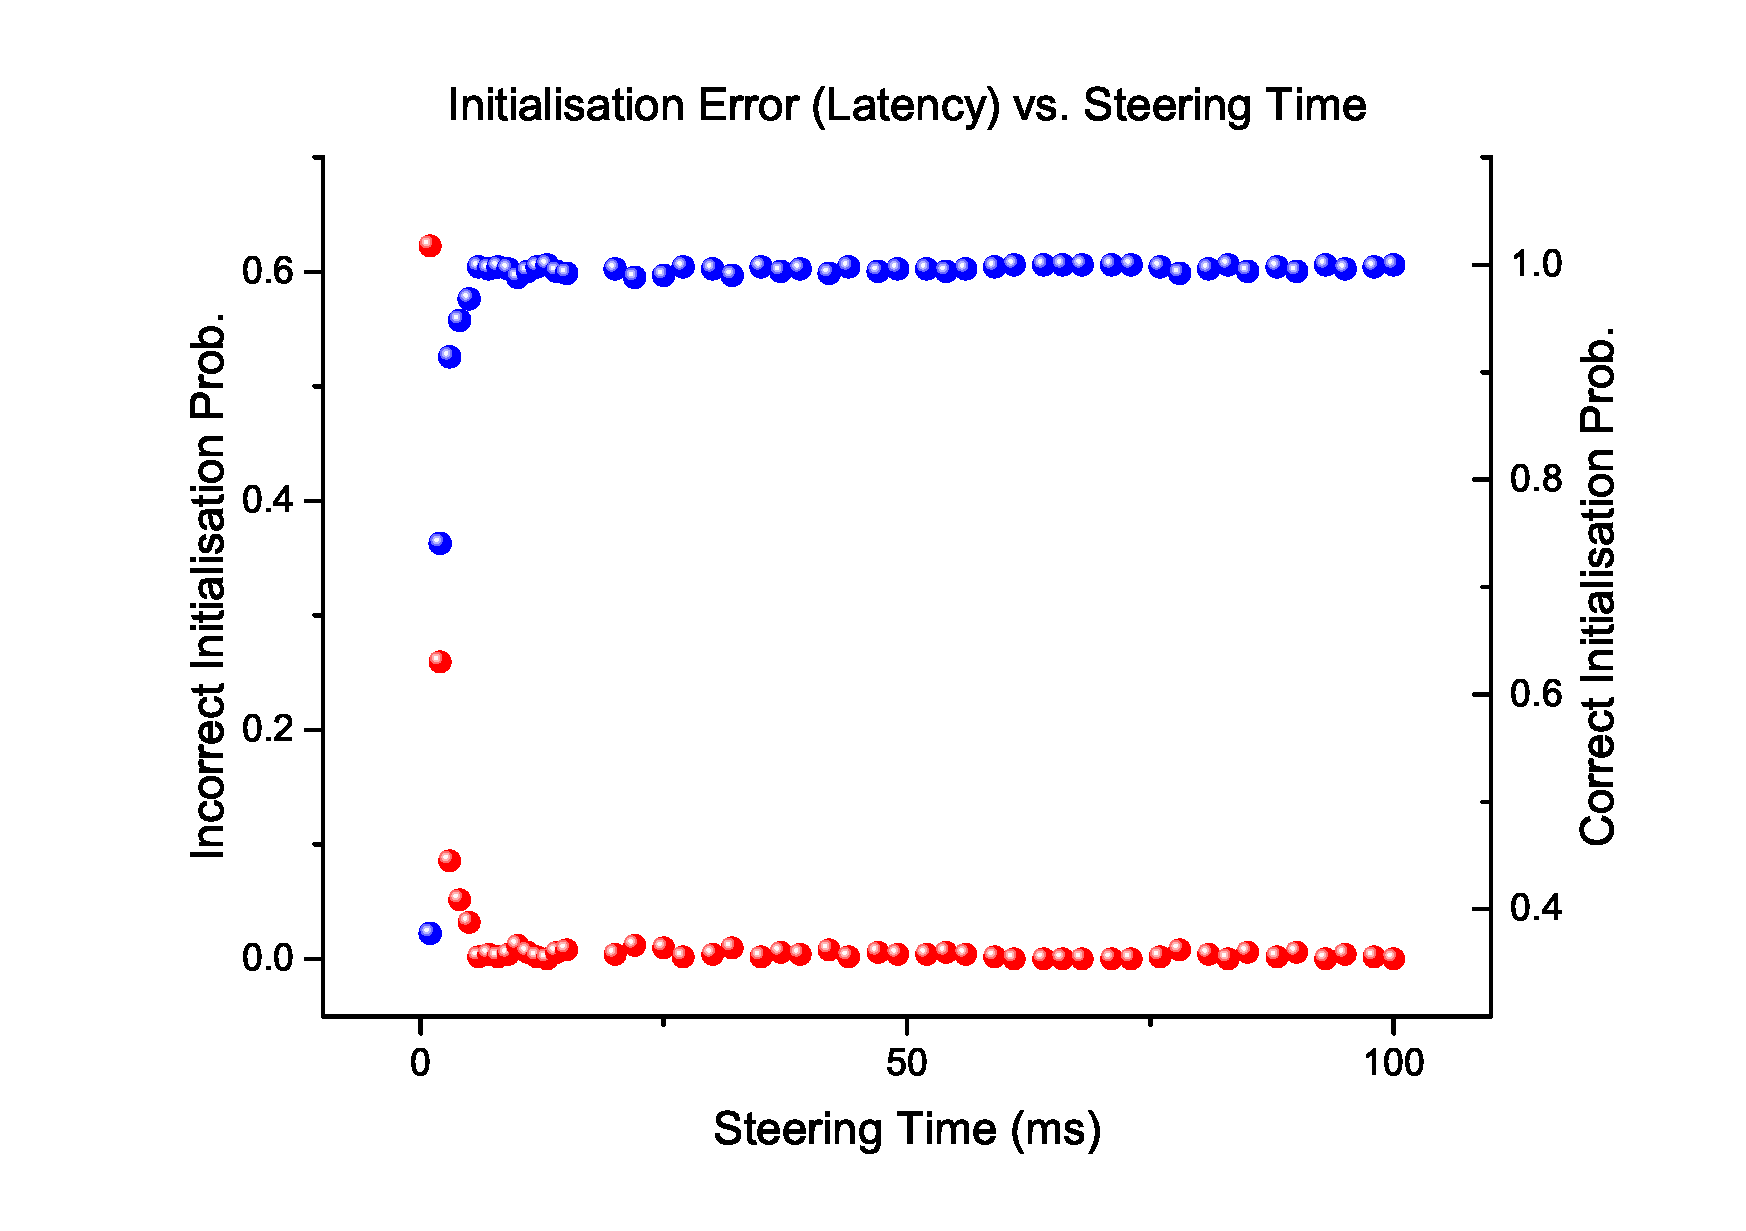
\includegraphics[width=\textwidth]{LatencyErrorFig}
		\caption{Probability of incorrect initialisation with varying steering times.}
		\label{fig::latency_errors}
	\end{figure}
	
	This has been the sole drive for further post-selection in the data, and for low steering times it has a significant effect however with longer steering times, the probability of an electron tunnelling off the donor diminishes, meaning there is a sharp decrease in latency errors. It is evident from the plots that after 6 ms of steering time, the probability of seemingly correct initialisation  is always greater than 98.8\%. Note that this is not a guarantee on the true state of the initialised electron, merely a guarantee that the initialisation scheme has run as expected. This confirms the reliability of a pre-selecting digital feedback loop, and holds room for improvement in mitigating the effect due to latency. The primary result from this analysis is that despite the potential for initialisation errors due to software to hardware latency, it is in fact a rare occurrence. This indicates pre-selection is far superior to post-selecting data that does not fit the required steering time, in terms of data economy. \todo{find out how much post-selection is done}
	
	There is a potential discrepancy between the observed, correct initialisation and the total experimental fidelity as a function of steering time. As noted in \hyperref[sec::steering]{Section \ref{sec::steering}}, the total fidelity only exceeds 98.8\% after a steering time of approximately 40 ms (Figure \ref{fig::wait_time}, 1.0 T), in contrast to 6 ms noted above. This discrepancy can be quashed when considering the long tunnel time at this magnetic field\todo{get a value for tunnel time}. While an initialisation may look correct, for small steering times relative to the tunnel time, the spin state will only be steered toward spin-down a small amount. Regardless of the number of correct or incorrect initialisations in this situation, the spin-state is poorly defined and therefore yields a poor total fidelity.
	